
\chapter{Overview of VB .\ NET and {\cs} .\ NET Language}


\section{Introduction to .\ Net Framework}

In computer (and software) programming, a framework is what is known as an abstraction where code can be altered to build application-specific software. The framework is a collection of Application Programming Interfaces, or APIs, that come with an enormous library of code that developers can use to write software, so they aren’t forced to write all the code from scratch.

An abstraction is basically the act of removing elements to reduce it to its essential form. In terms of software, it's the process of creating a clean slate for developers to work with.

.\ NET Framework is a software framework developed by Microsoft that runs primarily on Microsoft Windows. It includes a large class library named as Framework Class Library (FCL) and provides language interoperability (each language can use code written in other languages) across several programming languages. Programs written for .\ Net Framework execute in a software environment (in contrast to a hardware environment) named the \textit{Common Language Runtime (CLR)}. The CLR is an application virtual machine that provides services such as security, memory management, and exception handling. As such, computer code written using .\ NET Framework is called ``managed code". FCL and CLR together constitute the .\ NET Framework. 

FCL provides the user interface, data access, database connectivity, cryptography, web application development, numeric algorithms, and network communications.

%\subsection{.\ Net Framework Working Mechanism}
%.\ Net Languages Source Code are compiled into Microsoft Intermediate Language (MSIL).
%\begin{itemize}
%	\item MSIL we can call it as Intermediate Language (IL) or Common Intermediate Language (CIL). 
%	\item MSIL is a CPU independent set of instructions that can be converted to the native code. 
%	\item Metadata also created in the course of compile time with MSIL and stored it with the compiled code. \item Metadata is completely self-describing. 
%	\item Metadata is stored in a file called Manifest, and it contains information about the members, types, references and all the other data that the Common Language Runtime (CLR) needs for execution.
%\end{itemize}
%
%
%The Common Language Runtime (CLR) uses metadata to locate and load classes, generate native code, provide security, and execute Managed Code. Both Microsoft Intermediate Language (MSIL) and Metadata assembled together is known as Portable Executable (PE) file. Portable Executable (PE) is supposed to be portable across all 32-bit operating systems by Microsoft .\ Net Framework.
%
%During the runtime the Common Language Runtime (CLR)'s Just In Time (JIT) compiler converts the Microsoft Intermediate Language (MSIL) code into native code to the Operating System. The native code is Operating System independent and this code is known as Managed Code , that is, the language's functionality is managed by the .\ Net Framework . The Common Language Runtime (CLR) provides various Just In Time (JIT) compilers, and each works on a different architecture depends on Operating Systems, that means the same Microsoft Intermediate Language (MSIL) can be executed on different Operating Systems. From the following section you can see how Common Language Runtime (CLR) functions .


\subsection{.\ Net Framework Architecture}
.Net Framework Architecture is a programming model for the .Net platform that provides an execution environment and integration with various programming languages for simple development and deployment of various Windows and desktop applications. It consists of class libraries and reusable components.
%%%%%%%%%%%%%%%%%%%%%%%%%%%%%%%%%%%%%%%%%%%
%										  %
%		Figure						  	  %
%										  %
%%%%%%%%%%%%%%%%%%%%%%%%%%%%%%%%%%%%%%%%%%%
\begin{figure}[ht!]
	\centering
	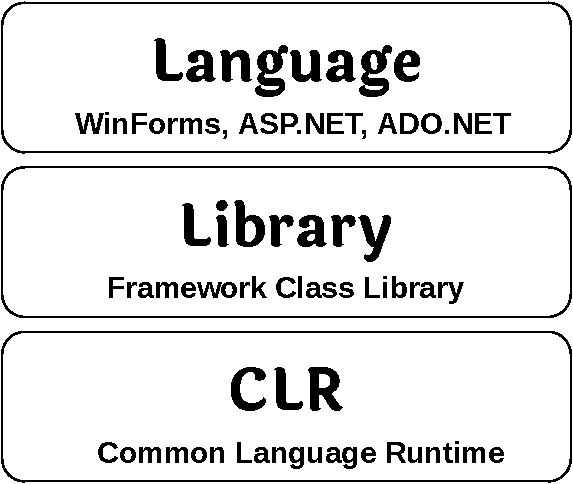
\includegraphics[width=0.7\textwidth]{dot-net-framework-architecture}
	\caption{.\ NET framework architecture}\label{fig:dot-net-architecture}
\end{figure}

The .\ Net Framework Architecture is the programming model for the .\ Net platform. It provides a managed execution environment, simplified development and deployment and integration with a wide variety of programming languages. The .\ Net Framework class library (FCL) is a comprehensive, object-oriented collection of reusable types that you can use to develop applications. The common language runtime (CLR) is the core runtime engine for executing applications in the .\ Net Framework. The CLR is fully protected from the outside environment and highly optimized within, taking advantage of the services that the CLR provides such as security, performance, deployment facilities, and memory management , including garbage collection.

%\subsubsection*{Components of .\ Net Framework}
%The .\ Net framework is composed of the following components:
%
%\begin{itemize}
%	\item \textit{ Common Language Runtime (CLR)}
%	\item \textit{Framework Class Library (FCL)} and
%	\item \textit{Languages (WinForms, ASP .\ NET, and ADO .\ NET, etc.\ )}.
%\end{itemize}
%
%
%\paragraph*{Common Language Runtime (CLR)}
%The Common Language Runtime (CLR) is an Execution Environment. It works as a layer between Operating Systems and the applications written in .\ Net languages that conforms to the Common Language Specification (CLS). The main function of CLR is to convert the Managed Code into native code and then execute the Program. The Managed Code compiled only when it needed, that is it converts the appropriate instructions when each function is called. CLR's Just In Time (JIT) compilation converts Intermediate Language (MSIL) to native code on demand at application run time.
%
%During the execution of the program, the CLR manages memory, Thread execution, Garbage Collection (GC), Exception Handling, Common Type System (CTS), code safety verifications, and other system services. The CLR defines the Common Type System (CTS), which is a standard type system used by all .\ Net languages. That means all .\ Net programming languages uses the same representation for common Data Types, so CLR is a language-independent runtime environment. The Common Language Runtime (CLR) environment is also referred to as a managed environment, because during the execution of a program it also controls the interaction with the Operating System.
%
%
%The CLR is an Execution Environment. Its main tasks are to convert the .\ Net Managed Code to native code, manage running code like a Virtual Machine and also controls the interaction with the Operating System.
%
%CLR manages Thread executions, Memory Management that is allocation of Objects and Buffers, Garbage Collection (GC) — Clean up the unused Objects and buffers, Exception Handling, CTS that is all .\ Net language that conforms to the Common Language Specification (CLS) have the same primitive Data Types, Code safety verification — code can be verified to ensure type safety, Language integration that is Common Language Runtime (CLR) follow a set of specification called Common Language Specification (CLS), this will ensure the interoperability between languages, Integrated security and other system services.
%
%\paragraph*{Framework Class Library (FCL)}
%The .\ Net Framework class library (FCL) provides the core functionality of .\ Net Framework architecture . The .\ Net Framework Class Library (FCL) includes a huge collection of reusable classes , interfaces, and value types that expedite and optimize the development process and provide access to system functionality.
%
%The .\ Net Framework class library (FCL) organized in a hierarchical tree structure and it is divided into Namespaces. Namespaces is a logical grouping of types for the purpose of identification. Framework class library (FCL) provides the consistent base types that are used across all .\ Net enabled languages. The Classes are accessed by namespaces, which reside within Assemblies. The System Namespace is the root for types in the .\ Net Framework. The .\ Net Framework class library (FCL) classes are managed classes that provide access to System Services . The .\ Net Framework class library (FCL) classes are object oriented and easy to use in program developments. Moreover, third-party components can integrate with the classes in the .\ Net Framework.
%
%


\subsubsection[CLR]{Common Language Runtime}
The ``Common Language Infrastructure'' or CLI is a platform in .\ Net architecture on which the .\ Net programs are executed.

The CLI has the following key features:

\begin{itemize}
	\item Exception Handling
	\item Garbage Collection
	\item Working with Various programming languages 
\end{itemize}

\subsubsection{Class Library}
The .NET Framework includes a set of standard class libraries. A class library is a collection of methods and functions that can be used for the core purpose.

For example, there is a class library with methods to handle all file-level operations. So, there is a method which can be used to read the text from a file. Similarly, there is a method to write text to a file.

Most of the methods are split into either the \texttt{System.*} or \texttt{Microsoft.* } namespaces\footnote{A namespace is a logical separation of methods.}. (The asterisk * just means a reference to all the methods that fall under the System or Microsoft namespace)



\subsubsection{Languages}
The types of applications that can be built in the .Net framework is classified broadly into the following categories

\begin{itemize}
	\item ADO.Net – This technology is used to develop applications to interact with Databases such as Oracle or Microsoft SQL Server: This is used for developing Forms-based applications, which would run on an end user machine. Notepad is an example of a client-based application.
	\item \texttt{ASP.Ne}t: This is used for developing web-based applications, which are made to run on any browser.
	\item \texttt{ADO.Net}: This technology is used to develop applications to interact with Databases such as Oracle or Microsoft SQL Server.
\end{itemize}



\subsection*{Common Language Specification (CLS)}
\begin{itemize}
	\item CLS is a set of basic language features that .\ Net Languages needed to develop Applications and Services, which are compatible with the .\ Net Framework.
	\item When there is a situation to communicate Objects written in different .\ Net Complaint languages, those objects must expose the features that are common to all the languages. 
	Common CLS ensures complete interoperability among applications, regardless of the language used to create the application.
	
\end{itemize}


\subsection*{Common Type System (CTS)}
CTS describes a set of types that can be used in different .\ Net languages in common. That is, the CTS ensure that objects written in different .\ Net languages can interact with each other. For Communicating between programs written in any .\ Net complaint language, the types have to be compatible on the basic level. 

These types can be Value Types or Reference Types. The Value Types are passed by values and stored in the stack. The Reference Types are passed by references and stored in the heap. CTS provides base set of Data Types which is responsible for cross language integration. The CLR can load and execute the source code written in any .\ Net language, only if the type is described in the CTS. Most of the members defined by types in the .\ Net FCL are CLS compliant Types.


\subsection*{Microsoft Intermediate Language (MSIL)}
\begin{itemize}
	\item MSIL stands for Microsoft Intermediate Language. 
	\item We can call it as Intermediate Language (IL) or Common Intermediate Language (CIL). 
	\item During the compile time, the compiler convert the source code into MSIL. 
	\item MSIL is a CPU-independent set of instructions that can be efficiently converted to the native code. 
	\item During the runtime the Common Language Runtime (CLR)'s Just In Time (JIT) compiler converts the MSIL code into native code to the Operating System.
\end{itemize}

When a compiler produces MSIL, it also produces Metadata. MSIL and Metadata are contained in a portable executable (PE) file. MSIL includes instructions for loading, storing, initializing, and calling methods on objects, as well as instructions for arithmetic and logical operations, control flow, direct memory access, exception handling, and other operations.

\subsection*{Just In Time Compiler (JIT)}
The .\ Net languages, which conforms to the Common Language Specification (CLS), uses its corresponding runtime to run the application on different Operating Systems. During the code execution time, the Managed Code compiled only when it is needed, that is it converts the appropriate instructions to the native code for execution just before when each function is called. This process is called Just In Time (JIT) compilation, also known as Dynamic Translation. With the help of Just In Time Compiler (JIT) the Common Language Runtime (CLR) doing these tasks.



The Common Language Runtime CLR provides various JIT compilers and each works on a different architecture depending on OS. That is why the same MSIL can be executed on different OS without rewriting the source code. JIT compilation preserves memory and save time during application initialization. 

\subsection*{Managed Code}
Managed Code in Microsoft .\ Net Framework, is the code that has executed by the Common Language Runtime (CLR) environment. On the other hand Unmanaged Code is directly executed by the computer's CPU. Data types, error-handling mechanisms, creation and destruction rules, and design guidelines vary between managed and unmanaged object models.

The benefits of Managed Code include programmers convenience and enhanced security. Managed code is designed to be more reliable and robust than unmanaged code, examples are Garbage Collection, Type Safety etc. The Managed Code running in a CLR cannot be accessed outside the runtime environment as well as cannot call directly from outside the runtime environment. This makes the programs more isolated and at the same time computers are more secure. Unmanaged Code can bypass the .\ Net Framework and make direct calls to the OS. Calling unmanaged code presents a major security risk.


\subsubsection*{Difference between managed and unmanaged code}
\paragraph*{What is Managed Code?}

Managed code is the code that is written to target the services of the managed runtime execution environment such as Common Language Runtime in .\ Net Technology.

\begin{figure}[ht!]
	\centering
	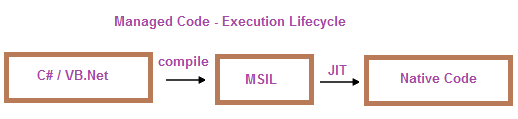
\includegraphics[width=0.7\linewidth]{managed-code}
	\caption[Managed Code]{Managed Code}
	\label{fig:managed-code}
\end{figure}

The Managed Code running under a CLR cannot be accessed outside the runtime environment as well as cannot call directly from outside the runtime environment. It refers to a contract of cooperation between natively executing code and the runtime. It offers services like garbage collection, run-time type checking, reference checking etc. By using managed code we can avoid many typical programming mistakes that lead to security holes and unstable applications, also, many unproductive programming tasks are automatically taken care of, such as type safety checking, memory management, destruction of unused objects etc.

\paragraph*{What is Unmanaged Code?}
Unmanaged code compiles straight to machine code and directly executed by the Operating System. The generated code runs natively on the host processor and the processor directly executes the code generated by the compiler. It is always compiled to target a specific architecture and will only run on the intended platform. If we want to run the same code on different architecture then we will have to recompile the code using that particular architecture.

Unmanaged executable files are basically a binary image, \texttt{x86} code, directly loaded into memory. This approach typically results in the fastest code execution, but diagnosing and recovery from errors might difficult and time-consuming in most cases. The memory allocation, type safety, security, etc needs to be taken care of by the programmer and this will lead unmanaged code prone to memory leaks like buffer overruns, pointer overrides etc.

All code compiled by traditional \texttt{C/C++} compilers are Unmanaged Code. COM components, ActiveX interfaces, and Win32 API functions are examples of unmanaged code. Managed code is code written in many high-level programming languages that are available for use with the Microsoft .\ Net Framework, including VB.\ Net, {\cs}, J{\texttt{\#}},  etc. Since Visual C++ can be compiled to either managed or unmanaged code it is possible to mix the two in the same application.


%\subsection*{.\ NET Components}
%The architecture of the .\ Net framework is based on the following key components:
%
%\subsubsection*{Common Language Runtime (CLR)}
%CLR handles execution of .\ NET code. The \textit{Common Language Infrastructure}
%or CLI is a platform on which the .\ Net programs are executed. It provides functionalities such as memory management, exception handling, debugging, security,
%thread execution, code execution, code safety, verification and compilation.
%
%The CLR also provides interoperability between different .\ Net languages. It
%provides a common environment for execution of different languages, such as {\cs},
%VB, VC++, etc.
%
%\subsubsection*{Class Library}
%The .\ Net Framework includes a set of standard class libraries. A class library is a collection of methods and functions that can be used for the core purpose.
%
%For example, there is a class library with methods to handle all file-level operations. So there is a method which can be used to read the text from a file. Similarly, there is a method to write text to a file.
%
%Most of the methods are split into either the \texttt{System.*} or \texttt{Microsoft.*} namespaces. (The asterisk \texttt{*} just means a reference to all the methods that fall under the System or Microsoft namespace)
%
%\subsubsection*{Languages}
%The types of applications that can be built in the .\ Net framework is classified broadly into the following categories.
%
%\paragraph*{WinForms}
%This is used for developing Forms-based applications, which would run on an end user machine. Notepad is an example of a client-based application.
%
%\paragraph*{ASP .\ NET}
%This is used for developing web-based applications, which are made to run on any browser such as Internet Explorer, Chrome or Firefox.
%	\begin{itemize}
%		\item The Web application would be processed on a server, which would have Internet Information Services Installed.
%		\item Internet Information Services or IIS is a Microsoft component which is used to execute an {Asp .\ Net} application.
%		\item The result of the execution is then sent to the client machines, and the output is shown in the browser.
%	\end{itemize}
%\paragraph*{ADO .\ NET}	
%This technology is used to develop applications to interact with Databases such as Oracle or Microsoft SQL Server.

%
%.\ NET Framework is designed to fulfill the following objectives:
%\begin{itemize}
%	\item To provide a consistent object-oriented programming environment whether object code is stored and executed locally, executed locally but web-distributed, or executed remotely.
%	
%	\item To provide a code-execution environment that minimizes software deployment and versioning conflicts.
%	
%	\item To provide a code-execution environment that promotes safe execution of code, including code created by an unknown or semi-trusted third party.
%	
%	\item To provide a code-execution environment that eliminates the performance problems of scripted or interpreted environments.
%	
%	\item To make the developer experience consistent across widely varying types of apps, such as Windows-based apps and Web-based apps.
%	
%	\item To build all communication on industry standards to ensure that code based on .\ Net Framework integrates with any other code.
%\end{itemize}
%
%
%
%\textbf{Features of .\ Net Framework}
%
%\begin{itemize}
%\item Less Coding and Increased Reuse of Code
%
%.\ Net framework supports Object-oriented programming (OOP) languages, which eliminates unnecessary codes and involves less coding. \.\ Net consists of reusable code and many reusable components. This translates into less time and consequently less cost to develop applications.
%
%\item Language-independent
%
%\.\ Net framework allows to develop Desktop, Web, Mobile and Console based applications. Also, it’s promoted as a language-independent framework, which means that development can happen in several compliant languages that include {\cs}, VB.\ Net, etc.
%
%\item Used for Service-Oriented Architecture
%
%.\ Net is often used for Web Services, WCF and Web API creation; which helps create REST API and SOAP based services that can communicate and transmit data utilizing standard Internet protocols.
%
%\item Easy Versioning \& Deployment Process
%
%With features like no-impact applications, private components, controlled code sharing, side-by-side versioning and partially trusted code, .\ Net framework makes deployment easier post development. The code execution environment supports safe code execution that minimizes software deployment and versioning conflicts. Moreover, it eliminates the performance problems of scripted or interpreted environments as well.
%
%\item Security
%
%.\ Net offers enhanced application security as web applications developed using ASP.\ Net have Windows confirmation and configuration. Managed code and CLR offer safeguard features like ‘role-based security’ and ‘code access security’.
%
%
%\item Multi-tiered Software Architecture
%
%.\ Net makes use of multi-tiered software architecture. It is known as multi-tiered because it physically separates functions for presentation, business logic and data management. It helps developers to build flexible applications. Moreover, developers also can add or edit a layer without being required to transform on the whole app.
%
%
%\item Feature-rich
%
%There are a variety of features which will be explored by the developers to make powerful apps. But then .\ Net Framework has been found to be a great platform for re-designing current applications in order to make it line up with the growing needs of an organization as well. For this, let us consider the case of its ‘rich toolbox’ and the ‘Designer’ in the visual studio. They let you access features such as automatic deployment, WYSIWYG editing, and drag-and-drop controls, etc. Any third-party control integration is also easily achievable with .\ Net Framework.
%
%\item Caching \& Exception Handling
%
%The caching \& exception handling features in .\ Net system, make your code more robust and easier-to-use.
%\end{itemize}

\subsection*{.\ Net Framework Design Principle}
The following design principles of the .\ Net framework is what makes it very relevant to create .\ Net based applications.

%\begin{description}
%	\item[Interoperability] The .\ Net framework provides a lot of backward support.
%	
%	\item [Portability].
%	
%	\item[Security]
%	
%	\item[Memory Management] The Common Language runtime does all the work or memory management. The .\ Net framework has all the capability to see those resources, which are not used by a running program. It would then release those resources accordingly. This is done via a program called the ``Garbage Collector" which runs as part of the .\ Net framework.
%	
%	The garbage collector runs at regular intervals and keeps on checking which system resources are not utilized, and frees them accordingly.
%	
%	\item[Simplified Deployment] The .\ Net framework also have tools, which can be used to package applications built on the .\ Net framework. These packages can then be distributed to client machines. The packages would then automatically install the application.
%\end{description}

The principal design features of Microsoft .\ Net Framework are:
\begin{multicols}{2}
\begin{itemize}
	\item \textit{Interoperability}
	\item \textit{Portability}
	\item \textit{Security}
	\item \textit{Language independence}
	\item \textit{Type safety}
	\item \textit{Memory management}
\end{itemize}
\end{multicols}


\subsubsection*{Interoperability}
Language interoperability is the ability of code to interact with code that is written using a different programming language. It can help maximize code reuse and, therefore, improve the efficiency of the development process. The .\ NET components can communicate with the existing COM components without migrating to those components into .\ NET. That means, this feature is a great help to reduce the migration cost and time. 

\subsubsection*{Portability}
 Applications built on the .\ Net framework can be made to work on any Windows platform. And now in recent times, Microsoft is also envisioning to make Microsoft products work on other platforms, such as iOS and Linux.
 
 \subsubsection*{Security}
  The .\ NET Framework has a good security mechanism. The inbuilt security mechanism helps in both validation and verification of applications. Every application can explicitly define their security mechanism. Each security mechanism is used to grant the user access to the code or to the running program.
  
  
 \subsubsection*{Language Independence}
 The .\ Net Framework is language independent. It is possible to use .\ Net from many programming languages because they have all agreed on some standards. This means that, as a programmer, we can develop in one of the many languages that target the .\ Net Framework, such as {\cs}, \texttt{C++/CLI}, Eiffel, F{\texttt{\#}, IronPython, IronRuby, PowerBuilder, Visual Basic, Visual COBOL, and Windows PowerShell. The .\ Net Framework presents a Common Type System (CTS) that characterizes every conceivable data sorts and programming builds bolstered by Common Language Runtime and how they might communicate with each other fitting in with CLI determination. Because of this feature, .\ Net Framework supports the exchange of types and object instances between libraries and applications written using any conforming .\ Net language.
 
 \subsubsection*{Type safety}
 Type-Safety is enforced by the CLR and the Language Compiler — in accordance to the CTS directives of the .\ Net Framework. Type-safe code cannot perform an operation on an object that is invalid for that object. This prevents ill-defined casts, wrong method invocations, and memory size issues when accessing an object. For example, if you have declared a variable as an integer, it cannot be assigned any value which is not an integer (by implicit conversion, or explicit conversion).
 
 \subsubsection*{Memory Management}
 The Common Language runtime does all the work or memory management. The .\ Net framework has all the capability to see those resources, which are not used by a running program. It would then release those resources accordingly. This is done via a program called the ``Garbage Collector", which runs as part of the .\ Net framework.
	
 The garbage collector runs at regular intervals and keeps on checking which system resources are not utilized, and frees them accordingly.
 

\section{Introduction to {\cs} and VB}
\subsection{{\cs}}
 {{\cs}} is a modern, general-purpose, object-oriented programming language developed by Microsoft and approved by European Computer Manufacturers Association (ECMA) and International Standards Organization (ISO).

{\cs} was developed by \textit{Anders Hejlsberg} and his team during the development of .\ Net Framework. It is based on C++ and Java, but it has many additional extensions used to perform component oriented programming approach.

{\cs} is designed for Common Language Infrastructure (CLI), which consists of the executable code and runtime environment that allows use of various high-level languages on different computer platforms and architectures.

\subsubsection*{{\cs} Features}
\begin{itemize}
	\item \textit{Simple}
	
	{\cs} is a simple language in the sense that it provides structured approach (to break the problem into parts), rich set of library functions, data types etc.
	
	\item \textit{Modern Programming Language}

	{\cs} programming is based upon the current trend and it is very powerful and simple for building scalable, interoperable and robust applications.
	\item \textit{Object-Oriented}
	
		{\cs} is object-oriented programming language. OOPs makes development and maintenance easier where as in Procedure-oriented programming language it is not easy to manage if code grows as project size grow.
		
	\item \textit{Type Safe}
	
	{\cs} type safe code can only access the memory location that it has permission to execute. Therefore it improves a security of the program.
	\item \textit{Interoperability}
	
	Interoperability process enables the {\cs} programs to do almost anything that a native C++ application can do.
	\item  Scalable and Updateable
	
	{\cs} is automatic scalable and updateable programming language. For updating our application we delete the old files and update them with new ones.
		
	\item \textit{Structured Programming Language}
	
	{\cs} is a structured programming language in the sense that we can break the program into parts using functions. So, it is easy to understand and modify.
	
	\item \textit{Rich Library}
	
	{\cs} provides a lot of inbuilt functions that makes the development fast.
	
\end{itemize}

%https://www.vbtutor.\ /lesson1.html
%Lesson 1 : Introduction to Visual Basic
%https://www.vbtutor.\ /lesson1.html
%2008 Dr.Liew Voon Kiong. 
\subsection{VB (Visual Basic) .\ NET}

Visual Basic is a third-generation event-driven programming language first released by Microsoft in 1991. It evolved from the earlier {DOS} version called {BASIC}. BASIC means \textit{Beginners' All-purpose Symbolic Instruction Code}. % Since then Microsoft has released many versions of Visual Basic, from Visual Basic 1.0 to the final version Visual Basic 6.0. Visual Basic is a user-friendly programming language designed for beginners, and it enables anyone to develop GUI window applications easily. 

VB .\ NET is a fully object-oriented programming language implemented in the .\ NET Framework. It was created to cater for the development of the web as well as mobile applications.

VB .\ Net is an update to Visual Basic that targets Microsoft .\ Net Framework. VB .\ Net has a lot of similarities to Visual Basic but also some differences. VB .\ Net is an object-oriented language, which supports the abstraction, encapsulation, inheritance, and polymorphism features. It is the most productive tool for rapidly creating a wide range of Windows, Web, Mobile, and Office applications built on the .\ Net Framework.

The Visual Basic language is designed to be human-readable and accessible to everyone from novice programmers to advanced system architects. All of this is built on top of the .\ Net Framework, which guarantees that programs written in Visual Basic run with unsurpassed scalability and reliability. The .\ Net Framework provides VB .\ Net programmers with the ability to create fully object oriented programs (OOPs), just like the ones created using Java, {\cs} or C\texttt{++}. Also programs written in VB.\ Net will interoperate seamlessly with programs written in any other .\ Net languages such as Visual {\cs}, Visual J\texttt{\#}, or Visual C\texttt{++}.

\subsubsection*{Featues of VB .\ Net}
VB .\ NET comes loaded with numerous features that have made it a popular programming language amongst programmers worldwide. These features include the following
\begin{multicols}{2}
\begin{itemize}
	\item VB.NET is not case-sensitive 
	\item It is an object-oriented programming language
	\item Garbage collection
	\item Events management
	\item Windows Forms
	\item Support for web application development
\end{itemize}
\end{multicols}


\section{Feature of Object Oriented Programming}

\subsection*{Object}	
Object is a collection of number of entities. Objects take up space in the memory. Objects are instances of classes. When a program is executed, the objects interact by sending messages to one another. Each object contain data and code to manipulate the data. Objects can interact without having know details of each others data or code.

\subsection*{Class}
Class is a collection of objects of similar type. Objects are variables of the type class. Once a class has been defined, we can create any number of objects belonging to that class. Classes are user define data types.
	 
\subsection*{Data Abstraction and Encapsulation}
 Combining data and functions into a single unit called class and the process is known as Encapsulation. Data encapsulation is important feature of a class. Class contains both data and functions. Data is not accessible from the outside world and only those function which are present in the class can access the data. The insulation of the data from direct access by the program is called data hiding or information hiding. Hiding the complexity of program is called Abstraction and only essential features are represented. In short, we can say that internal working is hidden.
	 
\subsection*{Dynamic Binding}
Refers to linking of function call with function definition is called binding and when it is take place at run time called dynamic binding.
	 
\subsection*{Message Passing} 
The process by which one object can interact with other object is called message passing.
	
\subsection*{Inheritance}
It is the process by which object of a class acquire the properties or features of objects of another class. The concept of inheritance provide the idea of re-usability means we can add additional features to an existing class without modifying it. This is possible by deriving a new class from the existing one. The new class will have the combined features of both the classes.

\subsection*{Polymorphism}
An operation may exhibit different behaviors in different instances. The behavior depends upon the types of data used in the operation. Its types:
 \begin{itemize}
 	\item Static / Compile Time Polymorphism.
 	\begin{itemize}
 		\item Method Overloading and 
 		\item Operator Overloading
 	\end{itemize}
 	\item Dynamic / Runtime Polymorphism.
 	
 \end{itemize}
 
\section{Scope of .\ Net  Technology}
Following are the scope of .\ Net Technology:
\begin{multicols}{2}
\begin{itemize}
		\item Cross platform mobile application development
		\item Desktop application
		\item Web application
		\item Web services
		\item Websites
		\item Games 
		\item Virtual Reality (VR) application
		\item Database application, etc.
\end{itemize}
\end{multicols}



